\documentclass[journal,twoside,web]{ieeecolor}
\usepackage{generic}
\usepackage{cite}
\usepackage{amsmath,amssymb,amsfonts}
\usepackage{algorithmic}
\usepackage[]{graphicx}
\usepackage{textcomp}
\usepackage{subfigure}
\usepackage{float}
\usepackage{hyperref}
\usepackage{lipsum}
\usepackage{multicol}
\usepackage{svg}
\usepackage{caption}
\usepackage[subrefformat=parens]{subcaption} 
%\usepackage[english, czech]{babel}
%\usepackage[useregional]{datetime2}
%\DTMsetdatestyle{czech}
\usepackage[ddmmyyyy]{datetime}
\def\BibTeX{{\rm B\kern-.05em{\sc i\kern-.025em b}\kern-.08em
    T\kern-.1667em\lower.7ex\hbox{E}\kern-.125emX}}
\markboth{ČESKÉ VYSOKÉ UČENÍ TECHNICKÉ V PRAZE, FAKULTA ELEKTROTECHNICKÁ, KATEDRA KYBERNETIKY, \today}
{ČESKÉ VYSOKÉ UČENÍ TECHNICKÉ V PRAZE, FAKULTA ELEKTROTECHNICKÁ, KATEDRA KYBERNETIKY, \today}


\hypersetup{
    colorlinks=true,
    linkcolor=blue,
    filecolor=magenta,      
    urlcolor=cyan,
    pdftitle={Semestrální úloha z předmětu Robotika},
    pdfpagemode=FullScreen,
    }
\begin{document}
\title{Úklid pracovního prostoru}
\author{Aleš Trna, Minh Hoang Tran \\ \begin{center}
        \today
    \end{center}
    \thanks{}}

\maketitle

\begin{abstract}
    Předmětem této práce je popis řešení závěrečné semestrální úlohy z předmětu Robotika.
\end{abstract}

\begin{IEEEkeywords}
    Robot, manipulátor, počítačové vidění
\end{IEEEkeywords}

\section{Zadání úlohy}
V pracovním prostoru robota CRS A465 jsou rozmístěny kostky o konstantní velikosti označené % CRS97 -> CRS A465
značkami typu \textit{Aruco}. Robot je umístěn v kleci, která vymezuje jeho pracovní prostor. %  na konstantním místě -> staticky
Ke kleci je staticky připevněna kamera, která snímá část pracovního prostoru. %zabírá stále stejnou scénu -> snímá část pracovního prostoru + odstranit tu část o pozici kamery
V pracovní scéně umístěny krabice, % vymazat "zároveň jsou"
které slouží k uložení kostek. Úkolem je správně roztřídit kostky s \textit{Aruco} %Naším úkolem je -> úkolem je správně 
značkami tak, aby kostky označené stejnými značkami byly uloženy na stejném místě (do stejné krabice).

\section{Vidění}
\subsection{Kalibrace kamery}
Abychom mohli detekovat, kde se kostky nachází, musíme provést kalibraci kamery. Kalibrací %Nacházejí -> nachází
kamery zjistíme distorzi, kterou poté budeme moci kompenzovat, pro jednoznačné %abychom dokázali -> pro
a přesné identifikování polohy \textit{Aruco} značky vůči kameře.\\
Princip kalibrace kamery spočívá v nafocení vzorků o známé velikosti a tvaru a následném porovnávání %přidat slovo "následném"
zkreslení výsledného obrázku s realitou. Pro jednoduchost se při této úloze obvykle používá
Šacovnice o konstantním rozměru čtverce. Pro naše řešení byla použita šachovnice
s \textit{Aruco} značkami na bílých polích o jiném, fixním rozměru díky které byla získána
přesnější data. Pro co nejpřesnější odhad distorze a parametrů kamery je třeba nafotit co nejvíce
vzorků z co nejvíce poloh a natočení šachovnice vůči kameře. %přidat "a natočení"
\begin{figure}[h!]
    \centering
    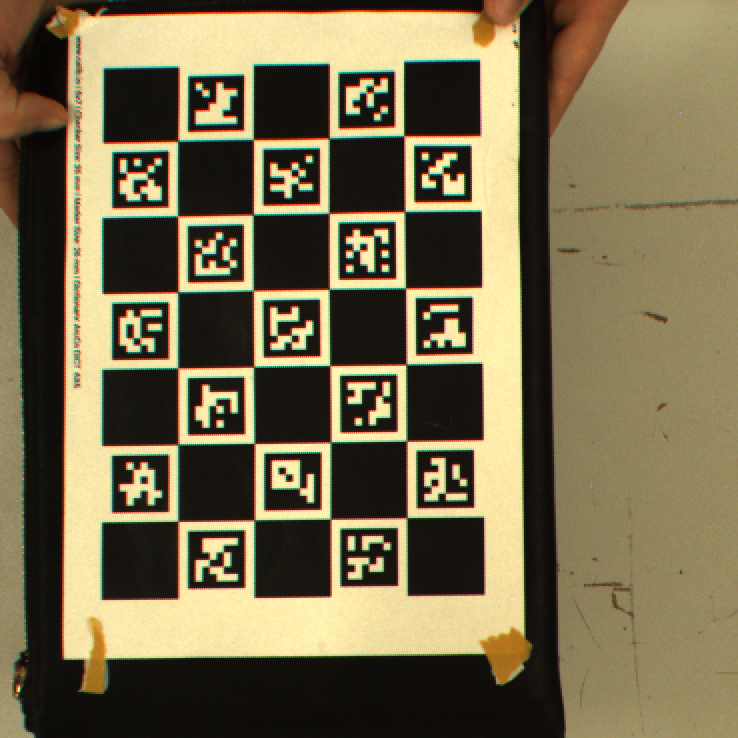
\includegraphics[width=0.45\linewidth]{images/CharucoFlat.png}
    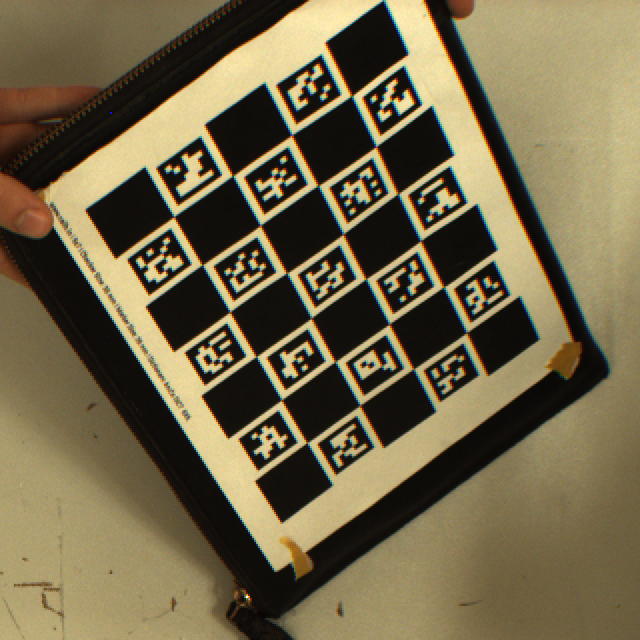
\includegraphics[width=0.45\linewidth]{images/CharucoSkewed.png}
    \caption{Plochá a nakloněná \textit{Charuco} deska}
    \label{fig:CharucoBoard}
\end{figure}\\
Na nafocených vzorcích byla detekována \textit{Charuco} deska pomocí funkce \textit{interpolateCornersCharuco}
z knihovny \textit{cv2}, díky které byla získána jednoznačná poloha rohů šachovnice a \textit{Aruco} značek. %chyba velké J v "Jednoznačná"
Tato data byla použita pro funkci \textit{CalibrateCameraCharuco} ze stejné knihovny.
Výsledkem byla matice kamery
\begin{equation}
    \mathbb{C} = \begin{pmatrix}f_x&0&c_x\\0&f_y&c_y\\0&0&1\end{pmatrix}
\end{equation}
Kde:
\begin{itemize}
    \item $f_x$, $f_y$ jsou ohniskové vzdálenosti v konkrétních osách\\
    \item $c_x$, $c_y$ jsou optické středy\\
\end{itemize}
Zároveň byly získány distorční koeficienty, díky kterým můžeme kompenzovat distorzi kamery. % Spojit do souvětí

\subsection{Hand to Eye kalibrace}
Ze zadání úlohy není jasné, kde přesně se kamera vůči robotovi nachází. Je mnoho způsobů, jak to zjistit.  %"několik -> mnoho
Nejjednodušší je změřit polohu kamery vůči pevně zvolenému bodu. Tato metoda je ale pro naše použití
příliš nepřesná. Dalším způsobem je vytvoření homografické matice, která by nám mapovala scénu kamery
do roviny. Předmětem této práce je však řešení nerovninného problému, proto tento způsob není vhodný.
Protože máme již zkalibrovaný obraz z kamery dokážeme díky funkcím knihovny \textit{cv2} zjistit polohu
objektů. Díky senzorům v robotu známe přesnou polohu chapadla vůči základně robota. V našem konkrétním případě
není kamera připevněna na chapadle robota, ale na konstrukci v konstantní poloze vůči robotu. %Nýbrž -> ale
Řešíme tedy "Hand to Eye" problém. Na jeho řešení můžeme využít opět knihovnu \textit{cv2}, konkrétně
funkci \hypertarget{cv2Handeye}{\textit{CalibrateRobotWorldHandEye}}. Do chapadla robota vložíme objekt o známých rozměrech,
u nějž můžeme zjistit jeho polohů vůči kameře. V našem případě využijeme kostku s \textit{Aruco} značkou.
S robotem budeme jezdit v zorném poli kamery a zaznamenávat scénu pomocí kamery a k ní korespondující
polohu chapadla vůči základně robota. Poté na fotkách detekujeme polohu \textit{Aruco} značek a data vložíme
do \hyperlink{cv2Handeye}{zmíněné funkce}. Řešíme tedy rovnici
\begin{equation}
    \mathbb{A}_i \mathbb{X} = \mathbb{Y}\mathbb{B}_i
\end{equation}
Kde:
\begin{itemize}
    \item $\mathbb{A}_i$ je $i$-tá naměřená transformace chapadla vůči bázi\\
    \item $\mathbb{X}$ je konstantní transformace značky vůči chapadlu robota\\
    \item $\mathbb{B}_i$ je $i$-tá odhadnutá transformace značky vůči kameře\\
    \item $\mathbb{Y}$ je konstantní transformace kamery vůči bázi robota.
\end{itemize}
\begin{figure}[h!]
    \centering
    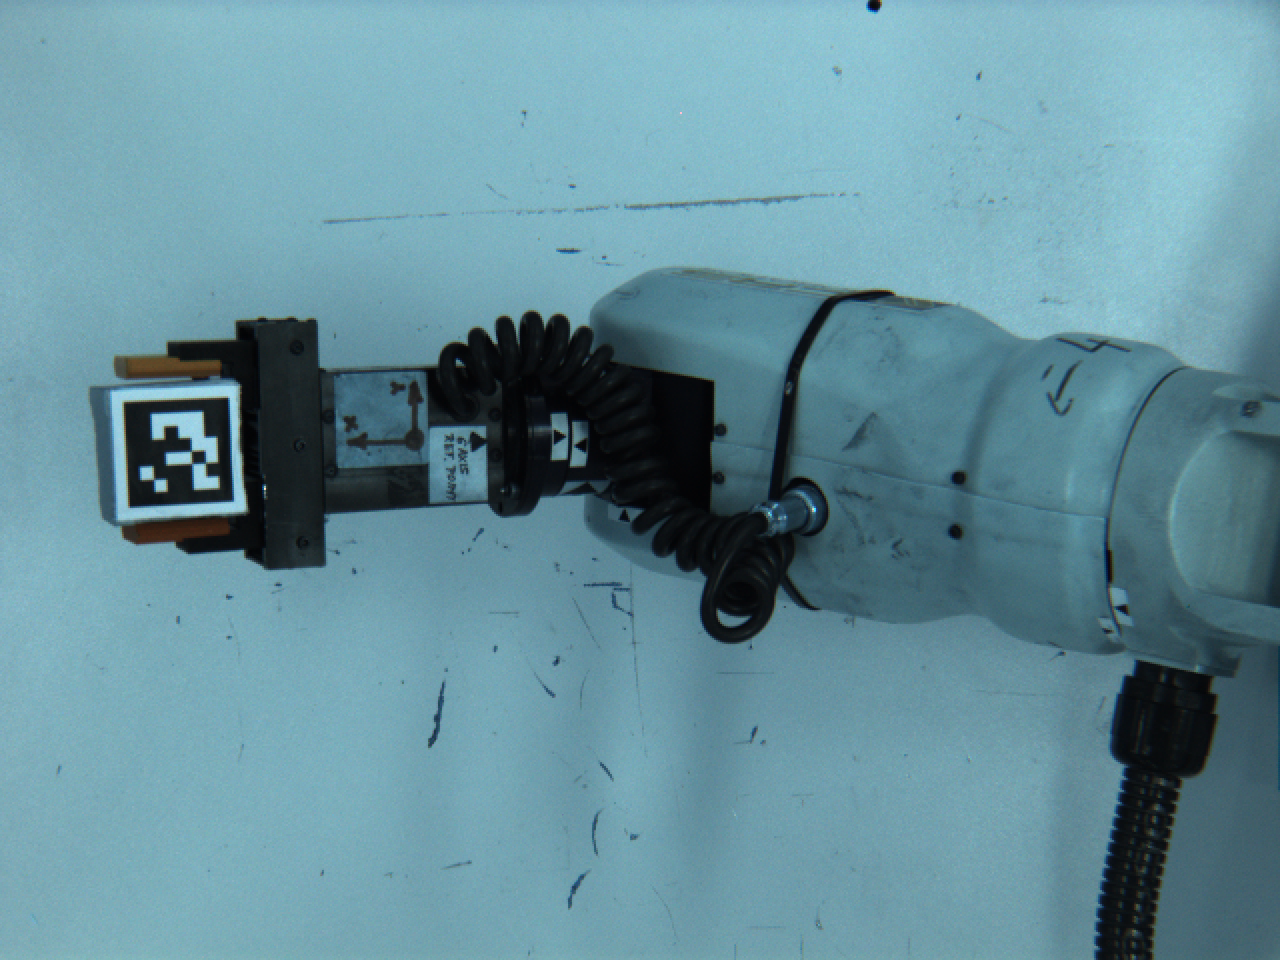
\includegraphics[width=0.8\linewidth]{images/Hand2eye.png}
    \caption{Kostka s \textit{Aruco} značkou uchopená (s konstantní transformací) v chapadle robota}
    \label{fig:ArucoInHand}
\end{figure}
Hledáme tedy transformaci $\mathbb{Y}$, pro její výpočet použijeme \hyperlink{cv2Handeye}{výše zmíněnou funkci}.

\subsection{Ověření správnosti transformace}
Po zjištění polohy kamery vůči základně robota můžeme zjistit polohu kostek vůči robotu. využijeme
k tomu rovnici
\begin{equation}
    T_{B\rightarrow K} = T_{B\rightarrow C} \cdot T_{C \rightarrow K}
\end{equation}
Kde:
\begin{itemize}
    \item $T_{B\rightarrow K}$ je transformace kostky vůči bázi robota\\
    \item $T_{B\rightarrow C}$ je transformace kamery vůči bázi robota\\
    \item $T_{C\rightarrow K}$ je transformace kostky vůči kameře\\
    \item Násobení tranformací odpovídá aplikování levé tranformace na transformaci pravou
\end{itemize}
Transformaci $T_{C\rightarrow K}$ získáme pomocí \textit{cv2.aruco} funkcí \textit{detectMarkers} a
\textit{estimatePoseSingleMarkers}. Jako ověření přesnosti kalibrace porovnáme změřenou a spočtenou
polohu kostek vůči bázi robota. A provedeme relativní pohyb kostkou v pracovním prostoru.
Dalším způsobem ověření bylo měření známých vzdáleností mezi více kostkami. % přidáno




\section{Návrh řešení}
Program je navrhnut jako stavový automat. Jeho zjednodušený vývojový diagram můžeme vidět na \hyperlink{diagram1}{obrázku 3}.
Jednotlivé stavy algoritmu podrobně rozebereme v této kapitole.
%Jako pokud se někdo podívá na kód (někdo kdo není Smutný/Krsek) tak zjistí, že to stavový automat není, ale v dokumentaci to zní lépe


\begin{figure}[h!]
    \centering
    \hypertarget{diagram1}{}
    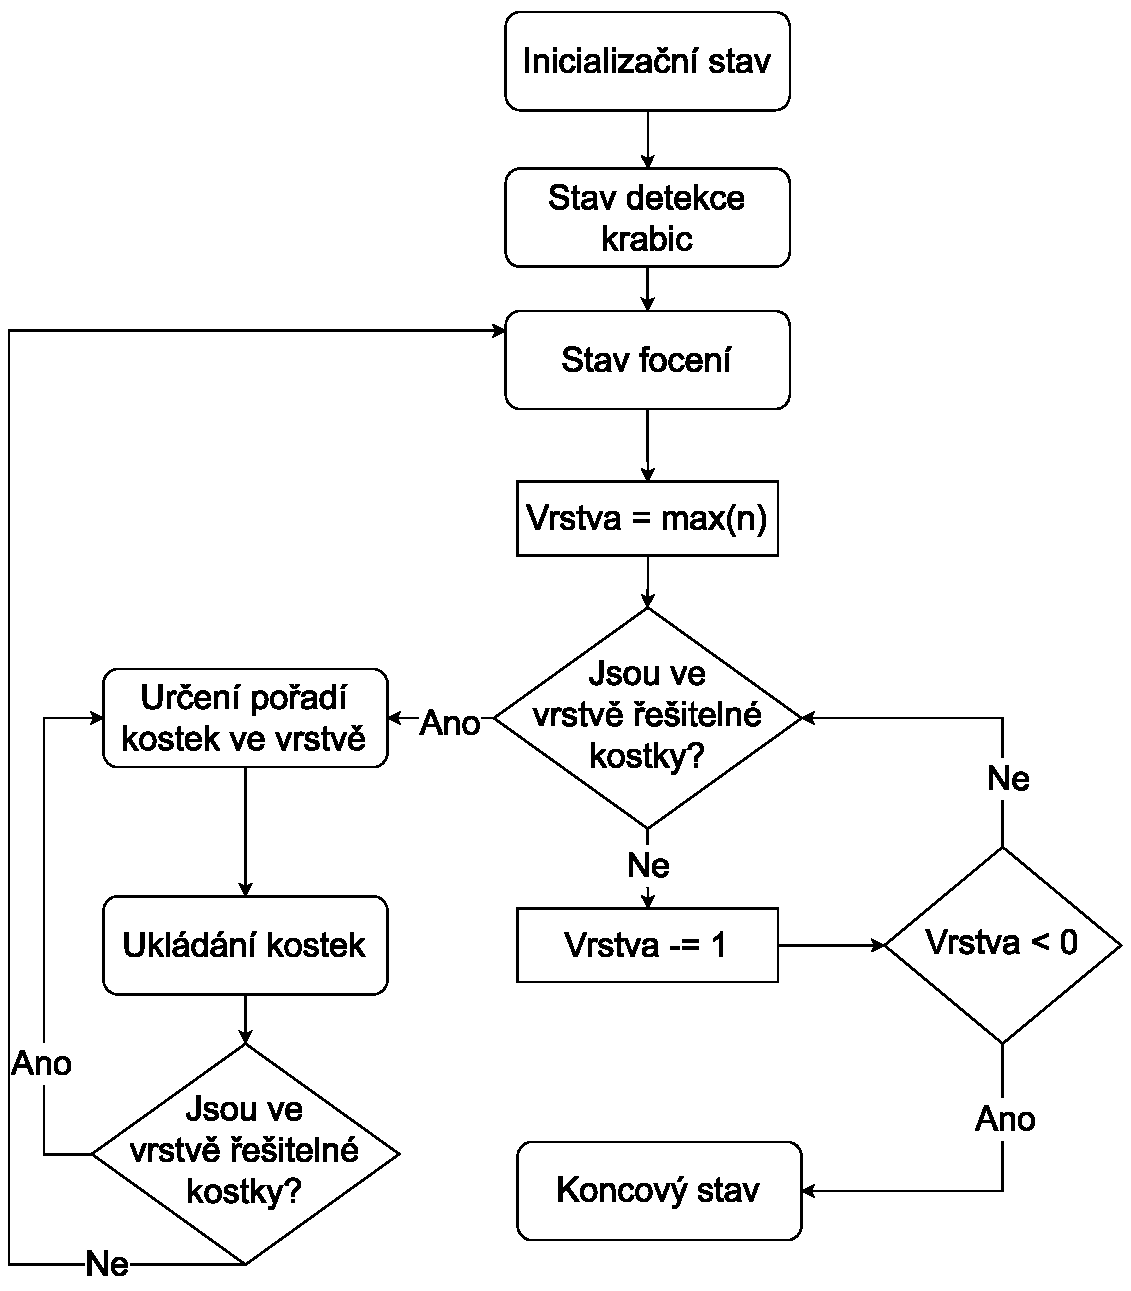
\includegraphics[width=\linewidth]{flowchart_cropped}
    \caption{Vývojový diagram popisující základní stavy stavového automatu}
    \label{fig:flowchart}
\end{figure}

\subsection{Inicializační stav}
Robot provede inicializaci chapadla a absolutní kalibraci polohy. Poté odjede do bezpečné pozice - tzv. "soft home".

\hypertarget{capturing_state}{\subsection{Stav focení}}
Robot se dostane do takové polohy, aby jeho ramena, nebo chapadlo nezasahovalo do zorného úhlu kamery. Protože
je kamera na fixním místě, můžeme pro toto použít absolutní polohu robota. Poté se zachytí fotografie scény pomocí
kamery na rámu robota. Tato fotografie je převedena do grayscale a podrobena funkcím z \textit{cv2}, které na ní detekují \textit{Aruco}
značky. Výstupem těchto funkcí je absolutní poloha značek vůči bázi robota. Polohy těchto značek jsou
diskretovány v ose \textit{z}, za účelem možnosti řešit problém po jednotlivých vrstvách - to znamená že kostky v první vrstvě dostanou
index 0, kostky ve druhé 1 atd...\\
Pokud jde o první stav focení od začátku běhu programu provede se zároveň \hyperlink{stav_detekce_krabic}{\textbf{Stav detekce krabic}}.

\hypertarget{stav_detekce_krabic}{\subsection{Stav detekce krabic}}
Protože id \textit{Aruco} značek krabic jsou odlišné od id značek kostek a tato id jsou předem známá, můžeme použít detekci krabic na
základě id značky. Při prvním focení programu se označí všechny detekované id z množiny id pro krabice jako "krabice". Předpokládá se přitom, že
jsou všechny dostupné krabice viditelné v zorném úhlu kamery od samého začátku běhu programu. K těmto krabicím jsou postupně přiřazovány id kostek,
které byly pozorovány. Pokud je v pracovním prostoru méně druhů kostek a více krabic budou všechny kostky stejného druhu uloženy do stejných krabic
a některé krabice zůstanou volné.
% Pokud naopak je v pracovním prostoru více druhů kostek a méně krabic, bude program rozdělovat kostky do krabic dokud
% bude mít volné krabice, jakmile volné krabice dojdou, začne skládat kostky druhu na něhož nezbyla krabice do krabice náhodně vybrané.
V druhém případě bude program přiřazoivat kostky ke krabicím s nejnižším počtem druhů již přiřazených kostek.
%oprava věty nad tímto commentem - chtělo by to možná formulovat lépe, idk
Všechny další kostky se stejným id budou přiřazeny do stejné krabice. % tady změna
% Přiřazení id krabice k id kostky je čistě náhodné. % smazat tuto větu -> zní blbě když mámě něco "náhodně" pokud to není přímo účelem
Po určení id krabic se uloží jejich pozice vůči bázi robota a kostky, jež do dané krabice patří se přesouvají na příslušné \textit{(x, y)} souřadnice.

Způsob, jak se předchází detekci již roztříděných kostek, řešíme měřením jejich vzdáleností v rovině \textit{xy} od jejich přiřazených krabic.
Je-li vzdálenost kostky od její přiřazené krabice menší než 100 mm, označuje program kostku jako roztříděnou a algoritmus pokračuje s další nalezenou kostkou.
Vzdálenost 100 mm jsme zvolili díky předem známým rozmerům krabice




\subsection{Třídění podle vrstev}
Pokud známe pozice krabic, můžeme se přesunout k třídění jednotlivých kostek. Po detekci a diskretizaci kostek v ose \textit{z} se vyberou se kostky
z nejvyšší detekované vrstvy a začne se řešit konkrétní vrstva. Zároveň se uloží nejvyšší vrstva kostky při startu programu. V rámci bezpečného, bezkolizního
pohybu robota všechny manipulace v rovině \textit{xy} probíhají nad touto vrstvou. Pokud současná nejvyšší vrstva neobsahuje kostku která by mohla být uchopena, %roztříděna -> uchopena
začne se hledat řešení o vrstvu níže. Tento proces se opakuje buď do nalezení řešitelné kostky, nebo dosažení nulté vrstvy.

\hypertarget{layer_sort}{\subsection{Pořadí kostek v jednotlivé vrstvě}}
Máme vybrané kostky z jedné konkrétní vrstvy kterou hodláme roztřídit. Nyní musíme určit pořadí, v jakém budeme kostky z dané vrstvy brát, a zároveň určit,
které kostky jsou řešitelné. Jako první filtr použijeme matici vzdálenosti, kterou sestavíme jako:\\
\begin{equation}
    \hypertarget{distance_matrix}{}
    \mathbb{D} = \begin{pmatrix}d_{1,1} & d_{1,2} & \dots  & d_{1, n} \\
               d_{2,1} & \ddots  &        & \vdots   \\
               \vdots  &         & \ddots & \vdots   \\
               d_{n,1} & \dots   & \dots  & d_{n, n} \\\end{pmatrix}
\end{equation}
kde $d_{i, j}$ je vzdálenost mezi kostkou s indexem $i$ kostkou a indexem $j$\\
Pokud na \hyperlink{distance_matrix}{matici vzdáleností} provedeme sumaci řádků (nebo sloupců, matice je symetrická), dostaneme součet vzdáleností všech kostek
od kostky na indexu i. Kostky budeme třídit právě podle tohoto kritéria. Budeme brát kostky od "nejvzdálenější" a pokud bude kostka uchopitelná roztřídíme ji. Takto budeme
postupovat až do té doby, než roztřídíme všechny kostky. Jak ale zjistíme, že je kostka uchopitelná a v jakém úhlu ji máme chytit? \\ %mít řečnickou otázku v dokumentaci mi nepřijde moc "odborné"
V našem řešení jsme využili toho že \textit{Aruco} markery jsou nesouměrné a můžeme tedy zjistit jejich rotaci vůči ose procházející kamerou.
U každé kostky najdeme v \hyperlink{distance_matrix}{matici vzdáleností} kostky, které jsou jejímu středu blíže než 70 mm.
Vytvoříme si dočasné "pole orientací", do kterého budeme ukládat relativní pozice kostek v blízkosti.
U všech těchto kostek spočítáme vektor transformace z naší kostky a vynormujeme jej. Spočítáme skalární součin tohoto vektoru
s orientací naší kostky (jednotkovým vektorem ve směru osy x) a jeho absolutní hodnotu porovnáme s hodnotou 0.70, která odpovídá skalárnímu součinu
jednotkového vektoru $\begin{pmatrix}\frac{1}{\sqrt{2}}&\frac{1}{\sqrt{2}}\end{pmatrix}$ - tedy jednotkové ose prvního a třetího kvadrantu. Pokud je hodnota
našeho skalárního součinu vyšší, uložíme do pole orientací 1, pokud ne, uložíme nulu. Toto provedeme pro všechny kostky, které jsou v okolí právě zkoumané kostky % okolo -> v okolí,  smazáno "naší"
menší než 70 mm.Pokud pole orientací obsahuje samé '1' víme, že kostku musíme chytnout z pohledu kamery "svisle", pokud samé '0', musíme kostku uchopit "vodorovně". %blíže -> menší
Pokud pole obsahuje jak '0' tak '1', víme, že kostku v současnosti nemůžeme uchopit (jako například kostku 2 na \hyperlink{cube_config}{obrázku 4}). Buď musíme nejdříve odstranit ostatní kostky, nebo jde o neřešitelnou úlohu.
Tato logika je vidět na \hyperlink{scalar_logic}{obrázku 5}. Protože absolutní hodnota skalárního součinu kostky "*" s kostkami 1 a 2 je větší, něž 0.7, je kostka "*"
uchopitelná "svisle". Toto je však pouze ukázkový příklad pro demonstraci logiky úchopu. Pokud by měl robot reálně řešit tuto situaci,
roztřídil by nejdříve kostky 1 nebo 2, protože součet vzdáleností od ostatních kostek je pro ně větší, než u kostky "*".
% overall tento odstavec zní těžko pochopitelně, ale nevím jak jinak to formulovat 
\begin{figure}[h!]
    \centering
    \hypertarget{cube_config}{}
    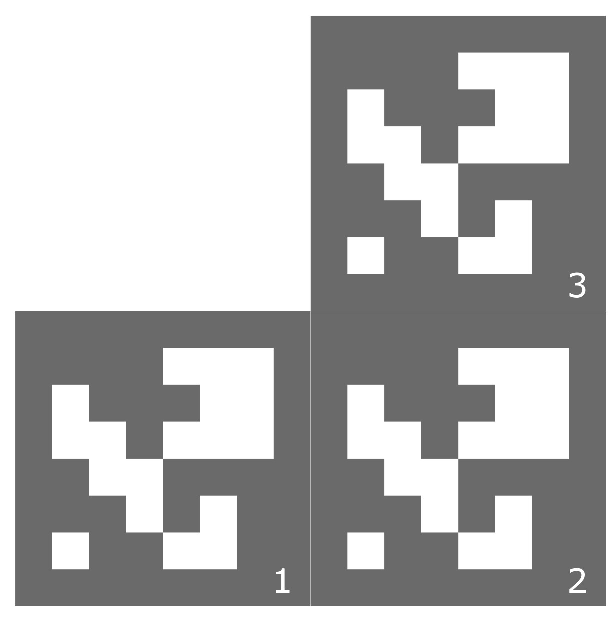
\includegraphics[width=0.8\linewidth]{images/neuchopitelna}
    \caption{Uchopitelné kostky 1,3 a neuchopitelná kostka 2 v dané konfiguraci kostek}
    \label{fig:cube_config}
\end{figure}\\

\begin{figure}[h!]
    \centering
    \hypertarget{scalar_logic}{}
    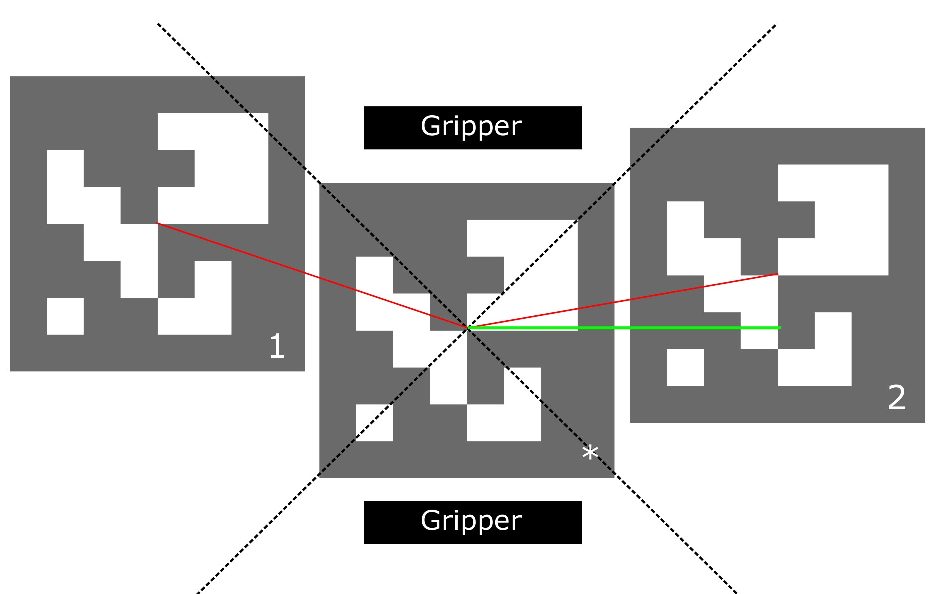
\includegraphics[width=\linewidth]{images/scalar}
    \caption{Logika úchopu kostky. Pro kostku "*" se provádí skalární součiny normovaných "červených vektorů"
        s normovaným "zeleným vektorem"}
    \label{fig:scalar_logic}
\end{figure}\\

\begin{figure}[h!]
    \centering
    \hypertarget{aruco_geometry}{}
    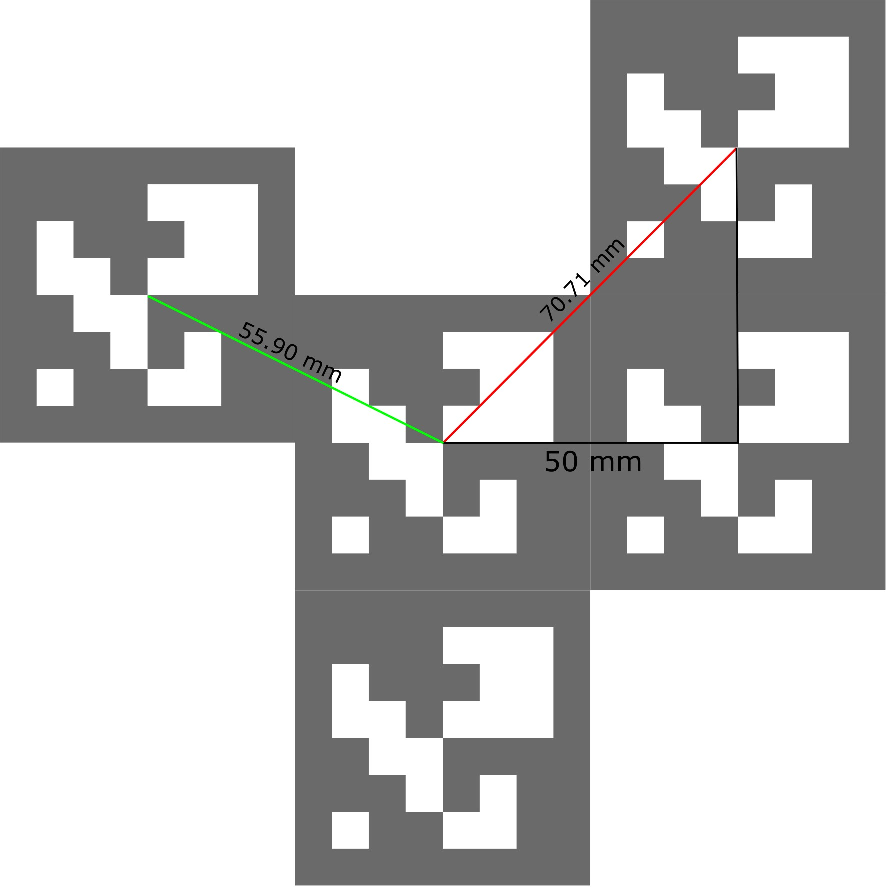
\includegraphics[width=0.8\linewidth]{aruco_geometry_cropped}
    \caption{Rozměry aruco kostek}
    \label{fig:aruco_geometry}
\end{figure}

\subsection{Třídění kostky}
Nyní, když máme určené pořadí, v jakém budeme kostky třídit, můžeme začít se samotným tříděním.
Ze \hyperlink{layer_sort}{stavu určujícího pořadí} máme přesnou polohu kostek a
pořadí, ve kterém je máme brát. Robot tedy podle tohoto pořadí nejdříve uchopí kostku na konkrétní pozici, vyjede
s ní nad nejvyšší detekovanou vrstvu při prvním focení a přemístí do předem určené krabice.
Do které krabice konkrétní kostka půjde je popsáno \hyperlink{stav_detekce_krabic}{zde}. Pokud leží kostka mimo dosah robota,
je vypsána chybová hláška, robot odjede do pozice "soft home" a je ukončen běh programu. Kostky jsou vždy uchopovány z vrchu, kolmo na
\textit{Aruco} značku.\\
Po roztřídění jedné kostky pokračuje podle pořadí daném ve \hyperlink{layer_sort}{stavu určujícího pořadí kostek} do té doby,
než všechny kostky roztřídí, nebo všechny zbývající kostky jsou neuchopitelné. Poté se přesune do \hyperlink{capturing_state}{stavu focení}.

\section{Komplikace při řešení úlohy}
\subsection{Neřešitelné vrstvy a virtuální kostky}
Pokud robot není schopen vyřešit nějakou vrstvu, bude podle \hyperlink{diagram1}{obrázku 3} postupovat do nižší vrstvy,
ve které bude dále postupovat podle výše popsaného algoritmu. Do této vrstvy však musíme doplnit "virtuální kostky",
o kterých robot neví, protože na nich stojí "neřešitelné" kostky z vyšší vrstvy. Tyto kostky označíme
jako rovněž neřešitelné, ale zbytek vrstvy budeme řešit podle stejného postupu. Na konci nám zbydou opět tyto "virtuální"
kostky plus jakékoli další "skutečné" kostky z této vrstvy. z nich opět vyrobíme "virtuální kostky", které
přidáme do nižší vrstvy.



\section{Původní způsoby řešení, od kterých sešlo}
\subsection{Opuštění zorného úhlu kamery}
Původně byla v návrhu řešení pro opuštění zorného úhlu kamery při focení použita poloha kloubů
$\begin{bmatrix}
        0 & 0 & 0 & 0 & 0 & 0
    \end{bmatrix}$, za účelem rychlosti řešení byla tato poloha předělána do fixní rotace nultého kloubu, který je schopen
násobně větší rychlosti, než všechny ostatní klouby robota. Před implementací tohoto řešení panovaly obavy, zda velké zrychlení v
jednom kloubu nemohou rozkalibrovat robota - tedy zda moment síly nebude moc velký. Naštěstí se prokázala tato obava jako neopodstatněná
a toto efektivnější řešení mohlo být použito.

\subsection{IKT a dosah robota}
Původně bylo řešení navrhnuto pouze na ukládání do krabic s tím, že kostka je ve kterékoli fázi pohybu vodorovná s rovinou stolu v pracovním prostoru
robota. Protože jsme však krabice umisťovali do rohů zorného úhle kamery, kde se občas stávalo, že poloha bylo mimo dosah robota, byla přidělána
funkce o ukládání v jakémkoli úhlu. Priorizována je opět poloha "kolmo na pracovní stůl",
nicméně pokud neexistuje konfigurace robota, ve které by této polohy byl schopen dosáhnout, vyhledá ve všech konfiguracích takovou polohu,
aby do krabice byl schopen kostku umístit.


\section{Závěr, diskuze a možnosti lepšího řešení}
Na této úloze jsme si vyskoušeli úlohu z praktické robotiky. Většina problémů při řešení vznikla při nastavování "vidění".
To, že tomu bylo tak i při takto jednoduché úloze objasňuje, proč se v moderní robotice jakýkoliv problém, který jde udělat bez vidění
řeší bez vidění. Nejpřekvapivější věc pro nás byla, že při vyšším počtu vzorků při kalibraci kamery a HandEye kalibraci bylo dosaženo
horších výsledků než s menším počtem vzorků.\\
Při testování jsme zjistili, že naše řešení kolabuje na testech, když se jedná o problém se 7 a více vrstvami,
protože kamera nedokáže přesně odhadnout polohu kostky v ose \textit{z}.
Současné řešení by se dalo vylepšit o kolizní funkci, která by umožňovala robotu hledat efektivnější trajektorie, a nezvedat kostky
nad úroveň té nejvyšší. Zároveň by se mohlo implementovat ukládání kostek do mřížky do krabic. Při testování jsme také přišli na to,
že by možná bylo lepší použít při počítání pořadí třídění kostek v dané vrstvě vždy jen kostky, které ještě nejsou roztříděné.
Tímto by se sice zvýšila výpočetní náročnost algoritmu, nicméně výsledky by byly nejspíše optimálnější. Dala by se také použít jiná metrika,
např. třídit kostku nejblíže od současné polohy robota.
\end{document}
